\documentclass[../dissertation.tex]{subfiles}
\begin{document}
The dissertation explored a few methods of untangling a curve.
In practice, however, we face untangling problem with ribbon-like objects as well,
which hold additional properties such as intrinsic curvatures, surface tension, and elasticity.

One could model this as a membrane $\Sigma$ and consider additional energy such as following\cite{mmb}:
\begin{equation}
    \mathcal{E}_{\Sigma} \coloneqq \iint_{\Sigma} \left( \gamma + 2 \kappa \left( H-H_0 \right)^2 + \bar \kappa K_g \right) \intd S
\end{equation}
where
\begin{itemize}
    \item $H$ and $K_G$ are the mean and Gaussian curvatures respectively.
    \item $\gamma$ is the surface tension.
    \item $\kappa$ and $\bar \kappa$ are the bending and saddle-splay modulus respectively.
    \item $H_0$ is the intrinsic mean curvature.
\end{itemize}
While formal definitions of the terms are out of scope of this dissertation,
by reducing $\tilde{\mathcal{E}_{\beta}^{\alpha}} + \mathcal{E}_{\Sigma} + \mathcal{C}$ where $\tilde{\mathcal{E}_{\beta}^{\alpha}}$ is generalised TPE for membranes,
one could easily conceive a numerical scheme for untangling, for example, DNA strands (Figure \ref{fig: DNA}) and by extension, tackling surface optimisation problems.

\begin{figure}[tbp]
    \centering
    %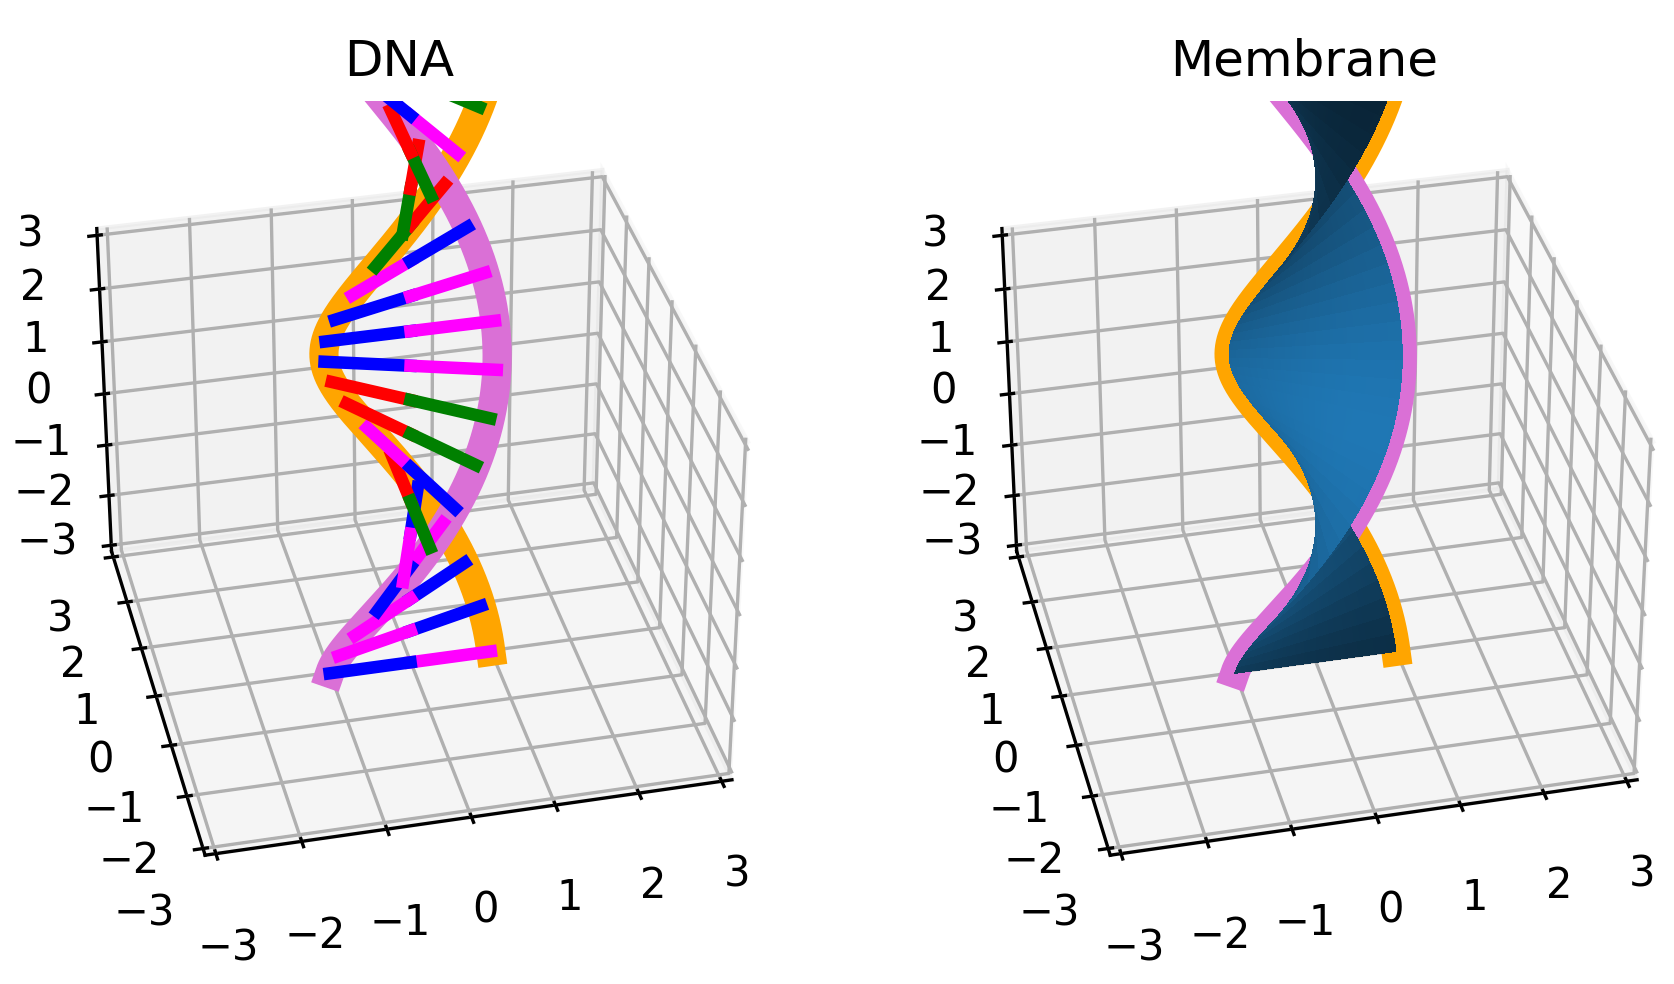
\includegraphics[width=\textwidth]{sections/MembraneImgs/dnaMembrane}
    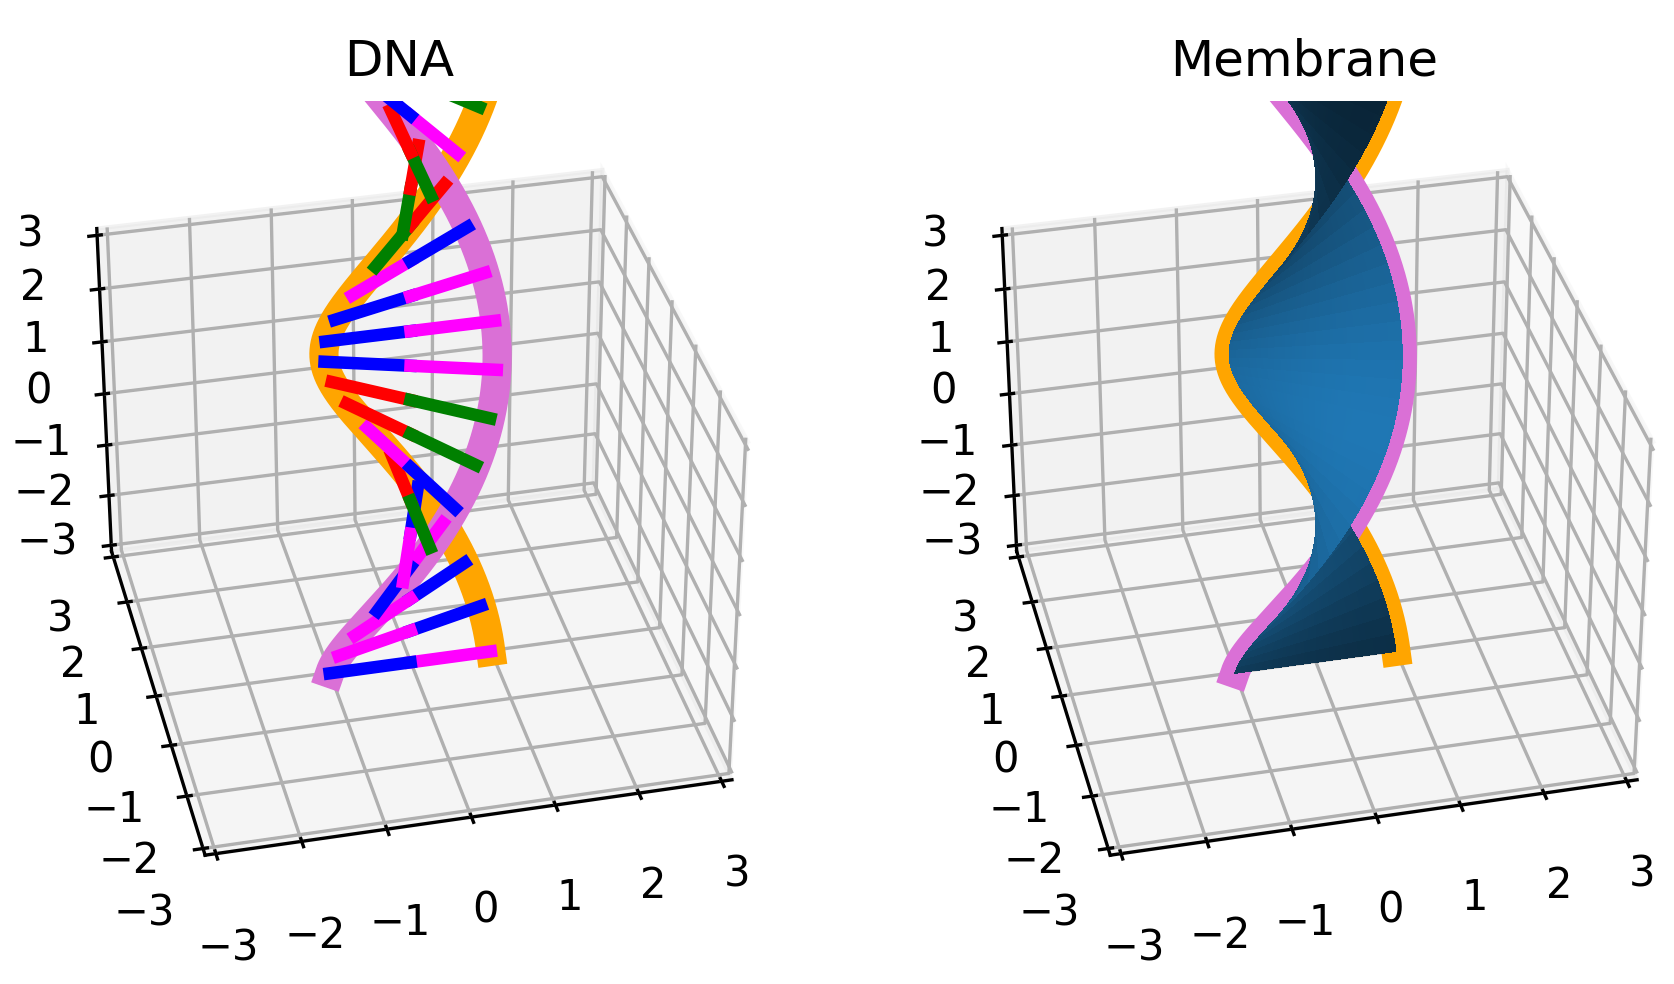
\includegraphics[scale=0.7]{sections/MembraneImgs/dnaMembrane}
    \caption{DNA is a ribbon-like structure which is often found wound around histone protein.\cite{gilchrist_2023}}
    \label{fig: DNA}
\end{figure}

%One could develop this into discussion of optimisation involving surfaces rather than curves.

\end{document}
